\documentclass{article}

\usepackage{geometry}
\usepackage{multicol}
\usepackage{fancyhdr}
\usepackage{lastpage}
\geometry{letterpaper,top=50pt,hmargin={20mm,20mm},headheight=15pt}
\usepackage{verbatim}
\usepackage{booktabs}
\usepackage{graphicx}
\usepackage{pgfplots}
\usepackage{lastpage}
\usepackage{float}
\usepackage{tikz}
\usepackage{amsmath}
\usepackage{listings}
\usetikzlibrary{shapes,arrows}
\definecolor{dark-green}{rgb}{0.0, 0.5, 0.0}


%%%<
%\usepackage[active,tightpage]{preview}
%%\PreviewEnvironment{tikzpicture}
%\setlength\PreviewBorder{5pt}%
%%%>
\pagestyle{fancy}

\fancypagestyle{first}{
\lhead{Final exam}
\chead{E213 - Thur, April 18, 2019}
\rhead{page~\thepage/\pageref{LastPage}}
\lfoot{} 
\cfoot{} 
\rfoot{}
}


\begin{document}
\lstset{numbers=left, numberstyle=\small, stepnumber=1, numbersep=5pt,language=python}

\pagestyle{first}
%\large{EOSC 213 Final Exam} \hspace{10cm} \large{April 18$^{\textrm{th}}$, 2019}
\large{Name:} \hspace{11cm} \large{ID: }
\begin{center}
\Huge{EOSC 213 - Final Exam}
\end{center}

\rule{\textwidth}{1pt}

\large{\textbf{Instructions (\textcolor{red}{XX} points in total)}}
\begin{multicols}{2}
\begin{itemize}
\item Don't panic (Douglas Adams, Hitchhiker's Guide to the Galaxy)
\item Read the examination before beginning.
\item Calculators are allowed (if you don't have one, just give the expression to type in a calculator).
\item You have exactly 90 minutes for the examination.
\item Be as precise and clear as possible.
\item This is a closed book examination.
\item If you get stuck, make an assumption, state what it is and try to carry on.
\end{itemize} 
\end{multicols}



\rule{\textwidth}{1pt}

\begin{description}
\item [Q0]  \textbf{[1 point]} Complete the sentence with your favourite word. \textit{Belgium is the most ....... country in the world.} 
\vspace{0.25cm}

\end{description}

%%%%%%%%%%%%%%%%%%%%%%%%%%%%%%%%%%%%%%%%%%%%%%%
%%%%%%%%%%%%%%%%%%%%%%%%%%%%%%%%%%%%%%%%%%%%%%%
%%%%%%%%%%%%%%%%%%%%%%%%%%%%%%%%%%%%%%%%%%%%%%%

\begin{description}
\item[Q1] \textbf{Acidity} is an important water-quality parameter at mine sites. It describes the moles of a base (typically carbonate) required to raise a water's pH to a prescribed value. Acidity is a \textbf{conserved quantity}. In practice, the units are moles of acidity per litre of water $[M/L^3]$.   


In this question, you will develop a model (equations) that describe the change in acidity over time in a tailings management facility (TMF or tailings pond), under these assumptions:
\end{description}

\begin{enumerate}
\item  the TMF has a total volume of $V(t)~[L^3]$, that changes in time in response to in- and outflows of water.
\item drainage from the pit flows into the TMF at a rate $Q_{pit}(t)~[L^3/T]$ with an acidity concentration of $c_{pit}~[M/L^3]$, measured in units of moles acidity per litre.
\item precipitation with zero acidity $c_{precip} = 0~ moles/l$ enters the TMF as precipitation on the surface of the TMF. Assume that the precipitation rate is given from data and can be represented in your model equations as $P(t),~[L/T]$ with units of $mm/day$. Assume that the surface area of the TMF is $A~[L^2]$ with units of $m^2$. Assume that area \textbf{does not change} as the volume in the TMF changes (an approximation that is valid for small changes in volume). 
\item evaporation removes water from the TMF at a rate that can be represented in your equation as $ET(t)~[L/T]$ with units of $mm/day$. 
\item the TMF is well stirred, such that the concentration of acidity in the TMF, $c_{TMF}~[M/L^3]$, measured in units of moles acidity per litre of water, is the same at all points in the pond at each instant in time.
\item water is discharged from the TMF at a rate $Q_{dis}(t)~[L^3/T]$ with an acidity concentration of $c_{TMF}$.
\item assume all other sources and sinks of water are negligible and can be ignored.

\end{enumerate}
 

\begin{table}[H]
  \caption{Summary of variables for Q1}
  \begin{center}
\begin{tabular}{lllll}
Variable & Description    & Dimension  \\
$V(t)$ &  Volume in the TMF                               & $[L^3]$ \\
 $Q_{pit}(t)$    & Rate of flow from pit into TMF      & $[L^3/T]$\\
 $c_{pit}(t)$     & Concentration of acidity in pit water & $[M/L^3]$\\
 $P(t)$            & Precipitation rate                       & $[L/T]$ \\
$ET(t)$          & Evaporation rate                    & $[L/T]$  \\
$A$               & Surface area of the TMF m           &$[L^2]$  \\
 $c_{TMF}(t)$ & Concentration of acidity in the TMF & $[M/L^3]$ \\
 $Q_{dis}(t)$   & Rate of discharge out of TMF      & $[L^3/T]$ 

\end{tabular}
\end{center}
\end{table}

\begin{description}
\item [Q1a] \textbf{[4 points]} Write a mathematical expression that describes how the volume of water in the TMF changes over a time interval from time $t$ to time $t+\Delta t$. That is, complete the following equation: 

$ V(t+\Delta t) - V(t) =$
\vspace{1.0cm}

\item [Q1b] \textbf{[2 points]}  Write the expression from part a) as a \textbf{differential equation} governing the rate of change of the water volume in the TMF. That is, complete the following equation:

${dV\over dt}=$
\vspace{1.5cm}
%\item [Q1c] \textbf{[4 points]}  Let $ACID(t)~[M]$ be the total mass of acidity in the TMF at time t. Write an expression for the change in acidity in the TMF over the time interval from time $t$ to time $t+\Delta t$. That is, complete this equation:

%$ACID(t+\Delta t) - ACID(t) = $
%\vspace{1.5cm}
\item [Q1c] \textbf{[5 points]}   Write a \textbf{differential equation}, or the \textbf{differential equations} that allow you to compute the \textbf{concentration} of acidity in the TMF $c_{TMF}(t)$ with time. 
\vspace{2.5cm}
\item [Q1d] \textbf{[2 points]} Provide a brief explanation for your answer to Q1c, or if you don't think you got the answer, how you think the problem should be approached.
\vspace{1.5cm}

%\item [Q1d] \textbf{[4 points]} Acidity can be generated from oxidation of pyrite in the tailings at the bottom of the pond. If the acidity flux per unit area of TMF bottom  $j_{acid}~[M/(L^2 T)]$ is given by $j_{acid} = k c_{TMF} + b$. What are the dimensions of the parameters $k$ and $b$?
%\vspace{1.5cm}

%%%%%%%%%%%%%%%%%%%%%%%%%%%%%%%%%%%%%%%%%%%%%%%
%%%%%%%%%%%%%%%%%%%%%%%%%%%%%%%%%%%%%%%%%%%%%%%
%%%%%%%%%%%%%%%%%%%%%%%%%%%%%%%%%%%%%%%%%%%%%%%

\end{description}


\rule{\textwidth}{1pt}



%%%%%%%%%%%%%%%%%%%%%%%%%%%%%%%%%%%%%%%%%%%%%%%
%%%%%%%%%%%%%%%%%%%%%%%%%%%%%%%%%%%%%%%%%%%%%%%
%%%%%%%%%%%%%%%%%%%%%%%%%%%%%%%%%%%%%%%%%%%%%%%

\begin{description}
\item [Q2] Finite - volume methods can be generalized from orthogonal N-S-E-W meshes to unstructured meshes. Below is a subsection from an \textbf{unstructured} finite-volume mesh. The gridblocks are labeled with their gridblock number. Because this is an unstructured mesh, the gridblock numbers do not follow a regular pattern as on a rectangular mesh. \par

\item[] \textbf{Notes:}
\begin{enumerate}
\item The mesh is a constant thickness $\Delta z$ (into the page).
\item The length of the interface between two gridblocks is given by $S_{i,j}$ where $i$, $j$ are two adjacent gridblocks that share an interface. For example, $S_{32,18}=S_{18,32}$ is the length of the interface between gridblocks 32 and 18, as indicated on the figure.
\item The distance separating nodes in adjacent gridblocks is given by the distance $dl_{i,j}$. For example as inidicated on the figure, the nodes in gridblocks 34 and 19 are separated by a distance $dl_{34,19}=dl_{19,34}$ .

\end{enumerate}
\item [Q2a] \textbf{[3 points]} Write a discrete appoximation for the mass flux rate by diffusion (non-porous media) between gridblocks 18 and 33, $J_{18,33}~[M/T]$. The component of specific diffusive flux in a direction $l$ is given by $j=-D{dc\over dl}$, where $dl~[L]$ is the distance in the $l$ direction and $D~[L/T]$ is the diffusion coefficient. This is the non-porous-media form of Fick's law.
\vspace{2.0cm}
\item [Q2b] \textbf{[3 points]} Write the finite-volume discrete approximation of the conservation equation for \textbf{steady-state} diffusion for gridblock 33 in terms of the concentration in gridblock 33, $c_{33}$,  the concentrations in the gridblocks adjacent to gridblock 33, $c_i$ (use the numbers given in the figure), the geometry of the mesh given by interfacial lengths, $S_{i,j}$, distance separating nodes, $dl_{i,j}$ and the thickness of mesh $\Delta z$. 

\end{description}
%%%%%%%%%%%%%%%%%%%%%%%%%%%%%%%%%%%%%%%%%%%%%%%
%%%%%%%%%      FIGURE OF MESH           %%%%%%%%%%%%%%%%%%%%%%%%%%
%%%%%%%%%%%%%%%%%%%%%%%%%%%%%%%%%%%%%%%%%%%%%%%

\begin{figure}[H]
  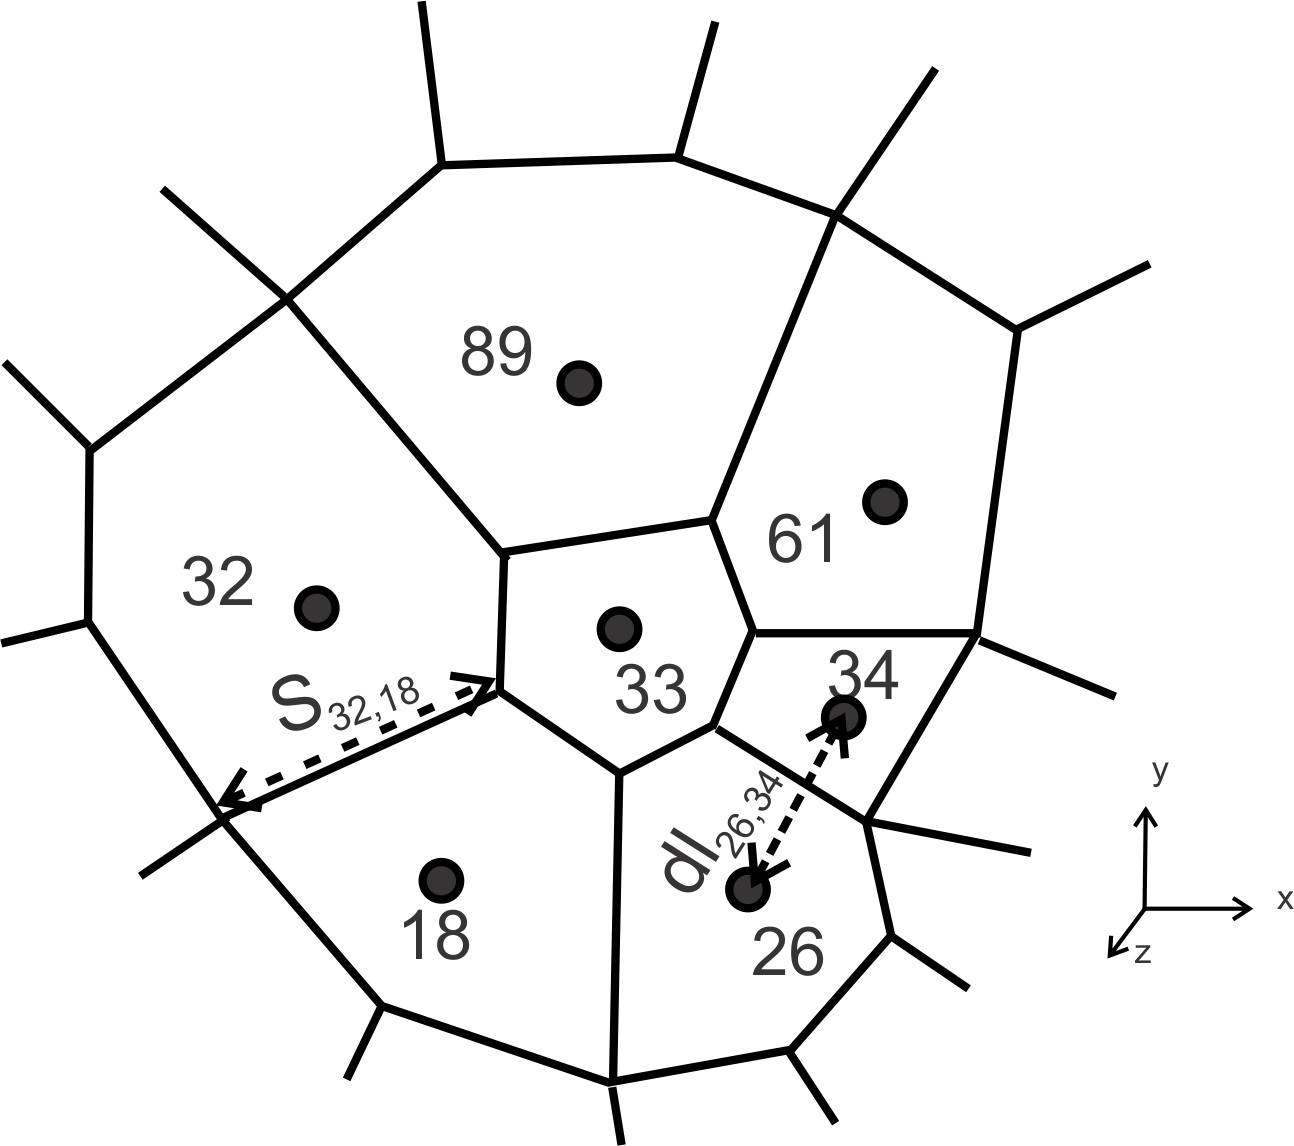
\includegraphics[scale=0.6]{unstructured_mesh2.png}
  \label{fig:grid}
\end{figure}
%%%%%%%%%%%%%%%%%%%%%%%%%%%%%%%%%%%%%%%%%%%%%%%
%%%%%%%%%      FIGURE OF MESH           %%%%%%%%%%%%%%%%%%%%%%%%%%
%%%%%%%%%%%%%%%%%%%%%%%%%%%%%%%%%%%%%%%%%%%%%%%

%%%\begin{description}
%%%\vspace{3cm}
%%%\item [Q1b] Write a first order discrete approximation of $\frac{dy}{dx}$ \textbf{[2 points]}
%%%\vspace{3.5cm}

%%%\item [Q1c] Write a second order discrete approximation of $\frac{dy}{dx}$ \textbf{[2 points]}
%%%\vspace{3.5cm}

%%%\end{description}

%%%\textbf{Question 1: ODE and finite-difference approximations}

%%%\begin{description}
%%%\item [Q1a] Write a discrete approximation of $\frac{d^2y}{dx^2}$ \textbf{[2 points]}
%%%\vspace{3cm}
%%%\item [Q1b] Write a first order discrete approximation of $\frac{dy}{dx}$ \textbf{[2 points]}
%%%\vspace{3.5cm}

%%%\item [Q1c] Write a second order discrete approximation of $\frac{dy}{dx}$ \textbf{[2 points]}
%%%\vspace{3.5cm}

%%%\end{description}

%%%Let us consider the following differential problem:

%%%\begin{equation}
%%%\left\lbrace
%%%\begin{array}{lll}
%%%\displaystyle{\frac{d^2y}{dx^2}} +6  \displaystyle{\frac{dy}{dx}} + 5y &=& 5x^2 + 2x \\
%%%y(0) &=& 2 \\
%%%y(3) & = & 5
%%%\end{array}
%%%\right. \label{eq:diffprob}
%%%\end{equation}

%%%\begin{description}
%%%\item [Q1d] Write the differential problem in a discrete approximation (using $x_i$ where $i$ refers the center of the gridblocks and $\Delta x$ is the distance between these centers) \textbf{[2 points]}
%%%\vspace{4.5cm}

%%%\end{description}

%%%A friend of yours used a computational method to solve the differential problem. Here are the results: 
%%%\begin{center}
%%%\begin{tabular}{|l|lllllll|}
%%%\hline
%%%$x$ & 0 & 0.5 &  1 & 1.5 & 2 & 2.5 & 3 \\ \hline
%%%$f(x)$ & 2  &  1.25  &  1  &  1.25 &   2 &    3.25 &    5  \\ 
%%%\hline
%%%\end{tabular}
%%%\end{center}

%%%\begin{description}

%%%\item [Q1e] Verify that the system of equations you wrote at Q1d is approximatively solved by the values given in the previous table. \textbf{[4 points]}
%%%\vspace{5cm}


%%%\item [Q1f] Prove that the function $y_1(x) = x^2-2x+2$ is a solution to the differential problem and that it satisfies the boundary conditions \textbf{[4 points]}
%%%\vspace{3cm}

%%%\item [Q1g] Give your friend feedback on her/his answer based on your previous answers.  \textbf{[2 points]}
%%%\vspace{3cm}


%%%\end{description}





%%%\begin{description}
%%%\item [Q1d] Using the answers of Q1a and Q1c, can you comment on the validity of his numerical answer? \textbf{[2 points]}
%%%\vspace{3cm}
%%%\item [Q1b] Compute a second-order approximation to the first derivative of the function $f(x)$ at $x = 2$.  \textbf{[2 points]}
%%%\vspace{3.5cm}

%%%\end{description}





%%%%%%%%%%%%%%%%%%%%%%%%%%%%%%%%%%%%%%%%%%%%%%%
%%%%%%%%%%%%%%%%%%%%%%%%%%%%%%%%%%%%%%%%%%%%%%%
%%%%%%%%%%%%%%%%%%%%%%%%%%%%%%%%%%%%%%%%%%%%%%%



\rule{\textwidth}{1pt}

\begin{description}


\item[Q3] Consider the following linear system which is the result of a finite-volume discretization of a physical problem:
%\begin{tabular}{ll}

\begin{equation}
A = \left( \begin{array}{cccccc}
    1 & 0 & 0 & 0 & 0 & 0 \\
    1 & -2 & 1 & 0 & 0 & 0 \\
    0 & 1 & -2 & 1  & 0 & 0 \\
    0 & 0 & 1 & -2 & 1  & 0 \\
    0 & 0 & 0 & 1 & -2 & 1  \\
    0 & 0 & 0 & 0 & -1 & 1 
\end{array}
\right) \quad B = \left( \begin{array}{c}
    1  \\
    0 \\
    -0.005 \\
    0  \\
    0  \\
    0  
\end{array} \right)  \quad Ax=B
\end{equation} 


\item [Q3a]  \textbf{[3 points]} Write the equations given by the first, second and last rows of the linear system. Write the equations in terms of the variables $x_0$, $x_1$, $\ldots$ (eg. the pythonic convention, with zero as the first index).

\vspace{2cm}
\item [Q3b]  \textbf{[2 points]} What is the dimension of the physical system represented by this system of equations: 1, 2 or 3 dimensional? To receive credit, you must explain your answer.  
\vspace{2cm}

\item [Q3c] \textbf{[2 points]} Which physical processes could be described by the linear system?  To receive credit, you must explain your answer.
\vspace{2cm}

\item [Q3d]  \textbf{[2 points]} Are there any source terms? If yes, specify where (and if it is a source (positive) or a sink (negative) source term).
\vspace{2cm}

\item [Q3e]  \textbf{[2 points]}  Describe the physical boundary conditions that are represented in this system. Refer to specific gridblock  numbers.
\vspace{2.0cm}



%\item [Q2i] Identify which of these 4 graphs is the asymptotic (final) solution to the presented problem. Give justifications as why the other ones are not compatible with the given system. If you don't know which one, try to describe the different results (what boundary conditions, ...). We assume that the medium is homogeneous: diffusion coefficient is the same everywhere. \textbf{[2 points]}
\end{description}

%\begin{tikzpicture}
%\begin{axis}[width = 7.5cm, xmin= 0 , xmax = 5, ymin = 0, ymax = 2, height = 7.5cm, grid = both, xlabel = x, legend pos = outer north east]
%\addplot[red, mark = o, mark size = 2 pt, line width = 0.1pt] table [x=x, y=a]{diff.txt}; \addlegendentry{(a)}
%\addplot[black, mark = square, mark size = 2pt, line width = 0.1 pt] table [x=x, y=b]{diff.txt}; \addlegendentry{(b)}
%\addplot[dark-green, mark = triangle, mark size = 2 pt, line width = 0.1pt] table [x=x, y=c]{diff.txt}; \addlegendentry{(c)}
%\addplot[blue, mark = diamond, mark size = 2pt] table [x=x, y=d]{diff.txt}; \addlegendentry{(d)}
%\end{axis}
%\end{tikzpicture}

\begin{description}

\item[Q4]  Pandas: consider the following dataframe  

\begin{verbatim}
  - Pandas learning objectives
#      - Be able to use the apply method to execute a function on every
#        row of a dataframe
#      - Be able to add a column to a data frame and use groupby with
#        that column to group dataframe rows into subset dataframes
#      - Be able to do simple statistics (mean, median, max, min,
#        summary) on dataframes and dataframe series
#      - Be able to construct dataframes from lists of tuples, lists of
#        dictionaries, or numpy arrays using from_records member
#        function
\end{verbatim}


  The following dataframe gives the temperature in deg C for 4 years, marked
  as either ``wet'' or ``driy''
  
\begin{lstlisting}[firstnumber=1]  
import pandas as pd
data=[[1970,2,14,22,10,'wet'],
      [1971,4,16,24,11,'dry'],
      [1972,6,18,26,12,'wet'],
      [1973,8,12,28,13,'wet']]
df=pd.DataFrame(data,
      columns=['year','djf','mam',
               'jja','son','precip'])
test.head()
\end{lstlisting}

\begin{tabular}{lrrrrl}
\toprule
{} &  djf &  mam &  jja &  son & precip \\
year &      &      &      &      &        \\
\midrule
1970 &    8 &    8 &    8 &    8 &      wet \\
1971 &    9 &    9 &    9 &    9 &      dry \\
1972 &   10 &   10 &   10 &   10 &      wet \\
1973 &   11 &   11 &   11 &   11 &      wet \\
\bottomrule
\end{tabular}

\item[Q4a] What does the following line print?

\verb+print(df.loc[1973,'djf'] - df.loc[1970,'son']+

\item[Q4b]

  Given the dataframe above, what does the following code fragment do?

\begin{verbatim}  
wet_dry=df.groupby('precip')
precip_dict={key:the_df for key,the_df in wet_dry}
\end{verbatim}  

  In your answer specify what the variables \verb+wet_dry+,
  \verb+precip_dict+ contain.  For \verb+precip_dict+ -- how many entries
  does it hold, and what are those entries?


\item[Q4c]

  How would you calculate the mean temperature of the wet seasons given \verb+precip_dict+?
  Your python doesn't have to execute, but it should unambiguously specify your
  intent.

  
\item[Q5] Classes and functions

\begin{verbatim}
# function/class learning objectives
2. Be able to define a simple class that contains class variables,
#    instance variables and instance methods and use it to pass parameters
#    into and out of a function.
#
# 3. Be able to write basic functions with default values (similar than
#    quiz 2)
#
\end{verbatim}

  
Consider the following class:
  
\begin{lstlisting}
import numpy as np
class hold_data:
    def __init__(self,nrows=2,ncols=2):
        self.data_array=np.zeros([nrows,ncols],dtype=np.float)

start_values = hold_data()
\end{lstlisting}

\item[5a] Class constructions

  What does the following python statement print?

\begin{verbatim}
print(start_values.data_array)
\end{verbatim}

\item[5b] Member functions

  Add a member function to \verb+hold_data+ called \verb+add_one+ that adds one to every element
  of \verb+start_values.data_array+ and show how you would call it.


\end{description}

\end{document}
%%% Local Variables:
%%% mode: latex
%%% TeX-master: t
%%% End:
